\documentclass{article}
\usepackage[utf8]{inputenc}
\usepackage[T2A]{fontenc}
\usepackage[russian]{babel}
\usepackage[normalem]{ulem}
\usepackage{amsfonts}
\usepackage{amsmath}
\usepackage{amsthm}
\usepackage{amssymb}
\usepackage{arcs}
\usepackage{fancyhdr}
\usepackage{float}
\usepackage[left=2cm,right=2cm,top=2cm,bottom=2cm]{geometry}
\usepackage{graphicx}
\usepackage{hyperref}
\usepackage{multicol}
\usepackage{stackrel}
\usepackage{xcolor}
\usepackage{cancel}

\makeatother
\makeatletter

\title{\textbf{Билеты к коллоку}}
\author{i.g. i.a.}
\date{20 марта 2023 г.}

\DeclareMathOperator*\lowlim{\underline{lim}}
\DeclareMathOperator*\uplim{\overline{lim}}

\newcommand*{\limToInf}[2]{\displaystyle \lim_{#1 \to \infty} #2}
\newcommand*{\limToZero}[2]{\displaystyle \lim_{#1 \to 0} #2}
\newcommand*{\lemma}[1]{\textbf{Лемма.} #1. \newline}
\newcommand*{\theorem}[2]{\textbf{Теорема #1. } #2 \newline}
\newcommand*{\definition}[1]{\textbf{Определение.} #1 \newline}
\newcommand*{\R}{\mathbb{R}}

\begin{document}
\tableofcontents
\maketitle

\section{Понятие первообразной. Теорема о двух первообразных. Понятие неопределенного интеграла.}

\textbf{Замечание: } Ниже под обозначением $\langle a, b \rangle$ будет пониматься произвольный промежуток: отрезок, интервал или полуинтервал.
\newline
\newline
\definition{Первообразной функции $f(x)$ на промежутке $\langle a, b \rangle$ называется функция $F(x)$ такая, что для всех $x \in \langle a, b \rangle$ выполняется равенство: }
$$
    F'(x) = f(x)
$$
\textbf{Несколько примеров: } 
\begin{enumerate}
    \item Пусть $f(x) = x^2$, тогда первообразная $F(x) = \cfrac{x^3}{3}$;
    \item Пусть $f(x) = \sin x$, тогда $F(x) = -\cos x$;
    \item Пусть $f(x) = 0$, тогда $F(x) = C$, $C \in \R$. 
\end{enumerate}
и так далее.
\newline 
\newline 
\theorem{(о двух первообразных)}{Пусть $F(x)$ - первообразная функция $f(x)$ на $\langle a, b \rangle$. Для того, чтобы $\Phi(x)$ также была первообразной для $f(x)$ на $\langle a, b \rangle$, необходимо и достаточно, чтобы}
$$
    F(x) - \Phi(x) \equiv C, \quad \forall x \in \langle a, b \rangle
$$
\begin{proof}
    Необходимость. Пусть $\Psi(x) = F(x) - \Phi(x)$, где $F(x), \Phi(x)$ - первообразные $f(x)$ на $\langle a, b \rangle$. Тогда $\forall x \in \langle a, b \rangle$:
    $$
        \Psi'(x) = (F(x) - \Phi(x))' = F'(x) - \Phi'(x) = f(x) - f(x) = 0
    $$
    По следствию из теоремы Лагранжа, для любых $x_1, x_2 \in \langle a,b \rangle$ таких, что $x_1 < x_2$
    $$
        \Psi(x_2) - \Psi(x_1) = \Psi'(\xi)(x_2 - x_1) = 0, \quad \xi \in (x_1, x_2) 
    $$
    тогда $\Psi'(x) \equiv const$
    \newline
    \newline 
    Достаточность. Пусть $F(x) - \Phi(x) = C$ выполнено, тогда $\Phi(x) = F(x) + C$ и тогда
    $$
        \Phi'(x) = F'(x) + C' = F'(x) + 0 = f(x)
    $$
    значит $\Phi(x)$ - первообразная $f(x)$ на $\langle a, b \rangle$.
\end{proof}
.
\newline
\definition{Неопределенным интегралом функции $f(x)$ на промежутке $\langle a, b \rangle$ называется \textit{множество всех первообразных на этом промежутке}. Обозначается:}
$$
    \int f(x)dx
$$
Также это значит, что 
$$
\int f(x)dx = F(x) + C
$$
\definition{Функция $F(x)$ называется \textit{обобщенной первообразной} $f(x)$ на $\langle a, b \rangle$, если $F(x)$ - непрерывна на $\langle a, b \rangle$ и $F'(x) = f(x)$ везде, кроме не более чем конечного числа точек.}
\section{Таблица неопределенных интегралов.}
\begin{figure}[!ht]
    \begin{center}
    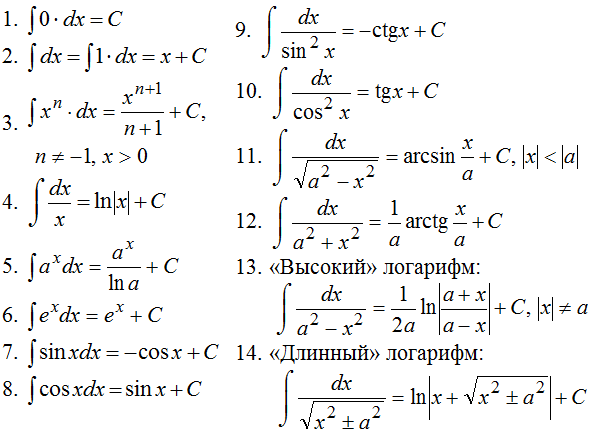
\includegraphics[scale=0.6]{unkn_inttbl.png}\caption{Таблица неопределенных интегралов.}\label{Таблица неопределенных интегралов.}
    \end{center}
\end{figure}
.\newline
Доказательство каждого из них состоит в том, что нужно продифференцировать правую часть\dots \textbf{!!ВЫУЧИТЕ ТАБЛИЦУ!!}
\section{Свойства неопределенного интеграла.}
ladies and gentlemans:
\begin{enumerate}
    \item \theorem{(связь с производной)}{Пусть $\int f(x)dx$ на $\langle a, b \rangle$, тогда на $\langle a, b \rangle$: }
    \begin{enumerate}
        \item $(\int f(x)dx)' = f(x)$;
        \item $d(\int f(x)dx) = f(x)dx$.
    \end{enumerate}
    \begin{proof}
        1, 2)
        $$
            \Bigl(\int f(x)dx \Bigr)' = (F(x) + C)' = f(x)
        $$
        Напомним, что $df = f'(x)dx$ и все становится очевидно.
    \end{proof}
    \item \lemma{Если $F(x)$ интегрируема на $\langle a, b \rangle$, то $\int dF(x) = F(x) + C$}
    \item \theorem{(линейность)}{Пусть на $\langle a, b \rangle$ существуют неопределенные интегралы $\int f(x)dx$ и $\int g(x)dx$, $\alpha^2 + \beta^2 \neq 0$. Тогда}
    $$
        \int (\alpha f(x) + \beta g(x))dx = \alpha\int f(x)dx + \beta\int f(x)dx
    $$
    \begin{proof}
        По предыдущему свойству,
        $$
            \Bigl(\alpha \int f(x)dx + \beta \int g(x)dx \Bigr)' = \alpha f(x) + \beta g(x)
        $$
        проинтегрировав обе части получим, что 
        $$  
            \alpha\int f(x)dx + \beta\int f(x)dx = \int (\alpha f(x) + \beta g(x))dx
        $$
    \end{proof}
    \item \theorem{формулы замены переменной}{Пусть на $\langle a, b \rangle$ существует неопределенный интеграл $\int f(x)dx, \; \varphi(t) \; : \; \langle \alpha, \beta \rangle \to \langle a, b \rangle$, дифференцируема на $\langle \alpha, \beta \rangle$, тогда}
    $$
        \int f(x)dx = \int f(\varphi(t))\varphi(t)dt 
    $$
    \begin{proof}
        Пусть $F(x)$ - первообразная для функции $f(x)$ на $\langle a, b \rangle$, тогда, согласно теореме о производной сложной функции, $F(\varphi(t))$ - первообразная для функции $f(\varphi(t))\varphi(t)$ на $\langle \alpha, \beta \rangle$, откуда и следует равенство.
    \end{proof}
    \item \theorem{формула интегрирования по частям}{Пусть $u, v$ - дифференцируемы на $\langle a, b \rangle$ и на этом промежутке существует неопределенный интеграл $\int vdu$, тогда на $\langle a, b \rangle$}
    $$
        \int vdu = uv - \int udv
    $$
    \begin{proof}
        $$
            (uv)' = u'v + uv'
        $$
        перейдем к дифференциалам
        $$
            d(uv) = udv + vdu \quad \Leftrightarrow \quad vdu = d(uv) - udv
        $$
        проинтегрировав (найдем первообразные) обе части получим требуемое.
    \end{proof}
\end{enumerate}
\section{Интегрирование рациональных дробей. Теорема о разложении на простейшие дроби и две леммы.}
% илья затехает
\section{Интегрирование простейших дробей}
% илья затехает
\section{Определение интеграла Римана. Пример неинтегрируеммой функции.}
\definition{ Говорят, что \textbf{разбиение $\tau$} введено на отрезке, если введена система точек $x_i, \; i \in \{0, 1, \dots, n\}$, удовлетворяющая условию: }
$$
    a = x_0 < x_1 < x_2 < \dots < x_n = b
$$
\textbf{Обозначения: }
$$
    \Delta x_i = x_i - x_{i-1}, \quad \Delta_i = [x_{i-1}, x_i], \quad i \in \{1, 2, \dots, n \}
$$
\definition{Величина $\lambda(\tau) = \displaystyle \max_{i \in \{1, 2, \dots, n \}} \Delta x_i$ называется \textbf{мелкостью(или рангом) разбиения(дробления)}.}
\newline
\definition{Говорят, что на отрезке введено \textbf{оснащенное разбиение} $(\tau, \xi)$, если на нем введено разбиение $\tau$ и выбрана система точек $\xi_i, \; i \in \{ 1, 2, \dots, n\}$, таким образом, что они находятся внутри $i$-ых отрезков.}
\newline
\definition{Пусть на отрезке задана функция $f(x)$ и введена разбиение $(\tau, \xi)$. Величина}
$$
    \sigma_\tau(f, \xi) = \sum_{i = 1}^{n} f(\xi_i) \Delta x_i
$$
называется \textbf{интегральная суммой} для функции $f(x)$ на отрезке.
\newline 
\newline 
\definition{Пусть функция $f(x)$ задана на отрезке $[a, b]$. Говорят, что число $I$ является \textbf{интегральном Римана} от функции $f(x)$ по отрезку $[a, b]$, если}
$$
    \forall \varepsilon > 0 \; \exists \delta \; : \: \forall \tau \; : \; \lambda(\tau) < \delta, \; \forall \varepsilon \; \Rightarrow |\sigma_\tau(f, \xi) - I| < \varepsilon
$$
при этом пишут 
$$
    I = \int_{a}^{b} f(x)dx
$$
\definition{Функция $f(x)$, для которой существует интеграл Римана на отрезке [a, b], называется \textbf{интегрируемой по Риману} на этом отрезке и обозначается $f \in R[a, b]$.}
\newline 
\subsection{Пример неинтегрируеммой функции.}
Например \textit{функция Дирихле}
$$
    d(x) = 
    \begin{cases}
        1, & x \in \mathbb{Q} \\
        0, & x \notin \mathbb{Q}
    \end{cases}
$$
не интегрируема ни на каком отрезке. Рассмотрим отрезок $[0, 1]$ и пусть $\tau$ - разбиение на нем.
\newline 
Выберем в каждом отрезке $\Delta_i$ точку $\xi_i \in \mathbb{Q}$. Тогда
$$
    \sigma_\tau(f, \xi) = \sum_{i = 1}^{n} d(\xi_i)\Delta x_i = \sum_{i = 1}^{n} \Delta x_i = 1
$$
Выберем в каждом отрезке $\Delta_i$ точку $\xi_i \in \mathbb{I}$. Тогда
$$
    \sigma_\tau(f, \xi) = \sum_{i = 1}^{n} d(\xi_i)\Delta x_i = \sum_{i = 1}^{n} 0\Delta x_i = 0
$$
Тем самым, устремляя мелкость разбиения к нулю, "предел" зависит от выбора средних точек $\xi$, что противоречит определению интеграла.
\newline 
\newline
\definition{Расширим определение интеграла:}
$$
    \int_{a}^{a} f(x)dx = 0
$$
$$
    \int_{b}^{a} f(x)dx = - \int_{a}^{b} f(x)dx, \quad a < b
$$
\section{Понятие сумм Дарбу, их свойства: неравенство для интегральной суммы, представления точными гранями, неравенства при измельчении разбиения, неравенства между верхней и нижней суммой для разных разбиений.}
\definition{Пусть функция $f(x)$ задана на отрезке [a, b] и $\tau$ - некоторое разбиение этого отрезка. Величины}
$$
    S_\tau(f) = \sum_{i = 1}^{n} M_i \Delta x_i, \quad M_i = \displaystyle \sup_{x \in \Delta_i}f(x)
$$
$$
    s_\tau(f) = \sum_{i = 1}^{n} m_i \Delta x_i, \quad m_i = \displaystyle \inf_{x \in \Delta_i}f(x)
$$
называют \textbf{верхней и нижней суммами Дарбу} для $f(x)$, отвечающими разбиению $\tau$, соответственно.
\newline\newline
\subsection{Очевидно, что $\dots$ aka неравенство для интегральной суммы.}  
Из определения нижней и верхней сумм дарбу очевидно: 
$$
    s_\tau(f) \leq \sigma_\tau(f, \xi) \leq S_\tau(f)
$$
\lemma{Ограниченность $f(x)$ сверху(снизу) равносильна конечности верхней(нижней) суммы Дарбу}
\begin{proof}
    Очевидно. 
    \newline 
    По хорошему, если функция $f(x)$ ограничена сверху, то ее супремум конечное число, и так как все супремумы на отрезках не больше супремума функции, \textit{очевидно}, что верхняя сумма Дарбу конечна.
\end{proof}
\subsection{Представление точными гранями.}
\lemma{Справедливы равенства}
$$
    S_\tau(f) = \displaystyle \sup_{\xi} \sigma_\tau (f, \xi), \quad s_\tau(f) = \displaystyle \inf_{\xi}\sigma_\tau(f, \xi) 
$$
\begin{proof}
    Докажем первое равенство. 
    \newline 
    \textit{Очевидно что...} $S_\tau(f) \geq \sigma_\tau(f, \xi)$. Пусть $f$ ограничена сверху на $[a, b]$. Пусть $\varepsilon > 0$ и по определению супремума
    $$
        \exists \xi_i \in \Delta_i \; : \; M_i - \cfrac{\varepsilon}{b - a} < f(\xi_i), \quad i = 1...n
    $$
    Домножим каждое неравенство на $\Delta x_i$ и сложим по $i$, получим
    $$
        \sum_{i = 1}^{n} \Biggl( M_i - \cfrac{\varepsilon}{b - a} \Biggr) \Delta x_i < \sum_{i = 1}^{n}f(\xi_i)\Delta x_i
    $$
    свернув в правой и левой части формулы получим
    $$
        S_\tau(f) - \varepsilon < \sigma_\tau(f, \xi)
    $$
    и так как $S_\tau(f) \geq \sigma_\tau(f, \xi)$:
    $$
        S_\tau(f) = \displaystyle \sup_{\xi} \sigma_\tau(f, \xi)
    $$
    по критерию супремума.
    \newline 
    Если $f$ не ограничена сверху на $[a, b]$, то она не ограничена хотя бы на одном подотрезке $[a, b]$. Для определенности рассмотрим такой подотрезок $\Delta_1$. Тогда на этом подотрезке супремумом будет являться $+\infty$, а тогда верхняя сумма Дарбу
    $$
        S_\tau(f) = \sum_{i = 1}^{n-1}M_i \Delta x_i + \infty = +\infty
    $$
    А так как любая интегральная сумма будет меньше чем $S_\tau(f)$, то $S_\tau(f) = \displaystyle \sup_{\xi}\sigma_\tau(f, \xi)$.
    \newline 
    Второе равенство доказывается аналогично.
\end{proof}
\subsection{Неравенства при измельчении разбиения.}
\definition{Пусть на отрезке [a, b] введенны разбиения $\tau_1$ и $\tau_2$. Говорят, что разбиение $\tau_1$ является \textbf{измельчением} разбиения $\tau_2$, если $\tau_2 \subset \tau_1$.}
\newline 
\lemma{Пусть $\tau_2 \subset \tau_1$, тогда}
$$
    S_{\tau_2}(f) \geq S_{\tau_1}(f), \quad s_{\tau_1}(f) \geq s_{\tau_2}(f)
$$
то есть при измельчении разбиения, верхние суммы Дарбу не увеличиваются, а нижние суммы Дарбу не уменьшаются.
\begin{proof}
    Достаточно доказать лемму для случая, когда измельчение $\tau_1$ получается из $\tau_2$ добавлением одной точки $\hat{x} \in (x_{k-1}, x_k)$. Тогда
    $$
        S_{\tau_2} = \sum_{i = 1}^{n} M_i \Delta x_i = \sum_{i = 1, i \neq k}^{n}M_i \Delta x_i + M_k \Delta x_k
    $$
    Пусть $M'_k = \displaystyle \sup_{x \in [x_{k-1}, \hat{x}]}f(x)$ и $M''_k = \displaystyle \sup_{x \in [\hat{x}, x_k]}f(x)$,
    $$  
        M_k \geq M'_k, \quad M_k \geq M''_k
    $$
    и далее распишем $M_k \Delta x_k$
    $$
        M_k \Delta x_k = M_k(\hat{x} - x_{k - 1}) + M_k(x_k - \hat{x}) \geq M'_k(\hat{x} - x_{k - 1}) + M''_k(x_k - \hat{x}),
    $$
    откуда (очевидно)
    $$
        S_{\tau_2}(f) \geq \sum_{i = 1, i \neq k}^{n} M_i \Delta x_i + M'_k(\hat{x} - x_{k - 1}) + M''_k(x_k - \hat{x}) = S_{\tau_1}(f)
    $$
    Второе неравенство доказывается аналогично.
\end{proof}
\subsection{Неравенство между верхней и нижней суммой Дарбу при различных разбиениях.}
\lemma{Пусть $\tau_1$ и $\tau_2$ - разбиения отрезка $[a, b]$, тогда}
$$
    s_{\tau_1}(f) \leq S_{\tau_2}(f)
$$
то есть любая нижняя сумма Дарбу не превосходит любой верхней суммы Дарбу.
\begin{proof}
    Пусть разбиениея $\tau = \tau_1 \cap \tau_2$ является разбиением отрезка $[a, b]$, причем $\tau_1 \subset \tau$, $\tau_2 \subset \tau$. По прошлой лемме и неравенстве между интегральными суммами и суммами Дарбу:
    $$
        s_{\tau_1}(f) \leq s_\tau(f) \leq S_\tau(f) \leq S_{\tau_2}(f)
    $$
    что \textit{очевидно} доказывает лемму.
\end{proof}
\section{Понятия интегралов Дарбу. Неравенство, связывающее суммы и интегралы Дарбу. Необходимое условие интегрируемости функции.}
\definition{Пусть функция задана и ограничена на $[a, b]$. Величины}
$$
    I^*(f) = \displaystyle \inf_{\tau}S_\tau(f), \quad I_*(f) = \sup_{\tau}s_\tau(f) 
$$
называются \textbf{верхним и нижним интегралами Дарбу} соответственно.
\subsection{Неравенство связывающее суммы и интегралы Дарбу.}
Для любых разбиений $\tau_1$ и $\tau_2$ отрезка $[a, b]$ выполнено неравенство
$$
    s_{\tau_1}(f) \leq I_*(f) \leq I^* \leq S_{\tau_2}(f)
$$
доказательство очевидно.
\subsection{Необходимое условие интегрируемости.}
Пусть $f \in R[a, b]$, тогда $f$ ограничена на $[a, b]$.
\begin{proof}
    Пусть $f$ не ограничена, например сверху. Тогда $S_\tau(f) = +\infty$ для любого разбиения $\tau$. Поэтому для любого числа $I$ и разбиения $\tau$ найдется такое оснащенное разбиение $(\tau, \xi)$, что
    $$
        \sigma_\tau(f, \xi) > I + 1
    $$
    то есть никакое число $I$ не является интегралом данной функции.
\end{proof}
\section{Критерии интегрируемости (Дарбу, Римана, через интегралы Дарбу). Запись с помощью колебания функции.}
\theorem{(Критерии интегрируемости)}{Пусть $f$ задана на $[a, b]$. Тогда следующие утверждения равносильны:}
\begin{enumerate}
    \item $f \in R[a, b]$;
    \item Критерий Дарбу:
    $$
        \forall \; \varepsilon > 0 \; \exists \delta > 0: \; \forall \tau \; \lambda(\tau) < \delta \Rightarrow S_\tau(f) - s_\tau(f) < \varepsilon
    $$
    \item Критерий Римана:
    $$
        \forall \; \varepsilon > 0 \; \exists \tau \; : \; S_\tau(f) - s_\tau(f) < \varepsilon
    $$
    \item 
    $$
        I_* = I^* \quad (= I)
    $$
\end{enumerate}
\begin{proof}
    \begin{itemize}
        \item Докажем $1 \Rightarrow 2$. Пусть функция $f(x)$ интегрируема на отрезке $[a, b]$ и $\varepsilon > 0$. Тогда 
        $$
            \exists \; \delta > 0: \; \forall \tau \; : \; \lambda(\tau) < \delta \; \forall \xi \quad \Rightarrow \quad |\sigma_\tau(f, \xi) - I| < \cfrac{\varepsilon}{3}
        $$
        откуда (раскрываем модуль)
        $$
            I - \cfrac{\varepsilon}{3} < \sigma_\tau(f, \xi) < I + \cfrac{\varepsilon}{3}
        $$
        перейдем к инфимуму и к супремуму в левой и правой части соответственно
        $$
            I - \cfrac{\varepsilon}{3} \leq s_\tau(f) \leq S_\tau(f) \leq I + \cfrac{\varepsilon}{3}
        $$
        откуда 
        $$
            S_\tau(f) - s_\tau(f) \leq \cfrac{2\varepsilon}{3} < \varepsilon    
        $$
        \item Переход $2 \Rightarrow 3$ очевиден, так как мы доказали для любого разбиения, а в критерии Римана сужение к "какому-то".
        \item Докажем $3 \Rightarrow 4$. Пусть $\varepsilon > 0$ и разбиение $\tau$ такое, что $S_\tau(f) - s_\tau(f) < \varepsilon$. Заметим, что тогда $f$ ограничена. Так как (из предыдущих свойств)
        $$
            s_\tau \leq I_* \leq I^* \leq S_\tau
        $$
        то $0 \leq I^* - I_* < \varepsilon$ для любого $\varepsilon$. То есть $I^* = I_*$.
        \item И докажем $4 \Rightarrow 1$. Пусть $I^* = I_* = I$. Тогда для $\varepsilon > 0$
        $$
            I_* = \displaystyle \sup_\tau s_\tau \quad \Rightarrow \quad \exists\tau_1 \; : \; s_{\tau_1} > I_* - \cfrac{\varepsilon}{4}
        $$
        $$
            I^* = \displaystyle \inf\tau S_\tau \quad \Rightarrow \quad \exists\tau_2 \; : \; S_{\tau_2} > I^* + \cfrac{\varepsilon}{4}
        $$
        %% илья дотехай пж
    \end{itemize}
\end{proof}
\subsection{Запись с помощью колебаний функции.}
\definition{Пусть функция $f(x)$ задана на множестве $E$. \textbf{Колебанием функции} на этом множестве называется величина}
$$
    \omega(f, E) = \displaystyle \sup_{x, y \in E}|f(x) - f(y)|
$$
И из определний супремума и инфимума легко получить 
$$
    \omega(f, E) = \displaystyle \sup_{x \in E}f(x) - \inf_{x \in E}f(x)
$$
И в критериях Дарбу и Римана можно заменить $S_\tau - s_\tau$
$$
    S_\tau - s_\tau = \sum_{i = 1}^{n}\omega_i(f)\Delta x_i
$$
\section{Свойства интегрируемых функций: линейность; интегрируемость произведения, частного, модуля; интегрируемость на меньшем отрезке и на склейке отрезков.}
Пусть $f(x), g(x) \in R[a, b]$, тогда 
\begin{enumerate}
    \item $\alpha f(x) + \beta g(x) \in R[a, b], \alpha, \beta \in \R$;
    \item $f(x)g(x) \in R[a, b]$;
    \item $|f(x)| \in R[a, b]$;
    \item Если $|f(x)| \geq C > 0$ на $[a, b]$, то $\cfrac{1}{f(x)} \in R[a, b]$;
    \item Пусть $[c, d] \subset [a, b]$, тогда $f(x) \in R[c, d]$.
\end{enumerate}
\begin{proof}
    \begin{enumerate}
        \item Так как
        $$
            |\alpha f(x) + \beta g(x) - \alpha f(y) - \beta g(y)| \leq |\alpha||f(x) - f(y)| + |\beta||g(x) - g(y)| \leq 
        $$  
        $$
            \leq |\alpha|\omega(f, E) + |\beta|\omega(g, E)
        $$
        то переходя к супремуму в левой части
        $$
            \omega(\alpha f + \beta g, E) \leq |\alpha|\omega(f, E) + |\beta|\omega(g, E)
        $$
        Пусть $\varepsilon > 0$. Так как $f \in R[a, b]$, перепишем критерий Дарбу через колебания
        $$
            \exists \delta_1 \; : \; \forall \tau: \; \lambda(\tau) < \delta_1 \Rightarrow \sum_{i = 1}^{n} \omega(f, \Delta_i)\Delta x_i < \cfrac{\varepsilon}{2(|\alpha| + 1)}        
        $$
        аналогично для $g$:
        $$
            \exists \delta_2 \; : \; \forall \tau: \; \lambda(\tau) < \delta_2 \Rightarrow \sum_{i = 1}^{n} \omega(g, \Delta_i)\Delta x_i < \cfrac{\varepsilon}{2(|\beta| + 1)}        
        $$  
        Пусть $\delta = min(\delta_1, \delta_2)$, тогда для любого $\tau$ такого, что $\lambda(\tau) < \delta$ выполняется
        $$
            \sum_{i = 1}^{n} \omega_i (\alpha f + \beta g)\Delta x_i \leq |\alpha| \sum_{i = 1}^{n} \omega_i(f)\Delta x_i + |\beta|
        $$
    \end{enumerate}
\end{proof}
\end{document}